% Results and performance analysis.
% Sources (repository paths):
%   simulation, seeds 1-5 ............ experiments/reports/2026-11-09-sim-main/
%   simulation, held-out seeds 6-10 .. experiments/reports/2026-11-09-sim-heldout/
%   calibration ablation (k = 1.109) . experiments/reports/2026-11-09-sim-heldout-k1.109/
%   static-fallback ablation ......... experiments/reports/2026-11-09-sim-static/
%   simulator calibration ............ experiments/reports/2026-11-09-sim-main/calibration.md
%   Mininet s2 after meter fix ....... experiments/reports/2026-10-26-mininet-s2-meter-fix/
%   Mininet s1-s3 + calibration ...... experiments/reports/2026-10-26-mininet-s1-s3-5seeds/
%   meter and idle-latency tests ..... experiments/reports/2026-10-26-meter-sweep/
% All simulation runs: commit 296d117 (code identical to c831a00, used for the Mininet s2 run).

% =====================================================================
\section{Results}
\label{sec:results}

\subsection{H1: prevention (simulation)}

Table~\ref{tab:sim} gives the main campaign. Only s2 and s6 separate the
controllers: s1, s3 and s4 produced no violations for any controller, and s5
produced violations in every slot for every controller. The held-out seeds 6--10
reproduced every pattern in the table (s2: 0.8 against 16.4 violation slots; s6:
1.8 against 16.4).

\begin{table*}[t]
\caption{Simulation, seeds 1--5: mean $\pm$ std per 60-slot run. ``Viol.'' = violation slots; ``Fb'' = fallback slots (of which uncertified); ``Shadow'' = applied actions the shield would have rejected; ``Res.'' = mean reserved bandwidth (Mbit/s).}
\label{tab:sim}
\centering
\footnotesize
\setlength{\tabcolsep}{3.5pt}
\begin{tabular}{@{}l|ccc|ccc|cc|cc|cc@{}}
\toprule
& \multicolumn{3}{c|}{shielded} & \multicolumn{3}{c|}{shielded-utility} & \multicolumn{2}{c|}{unshielded} & \multicolumn{2}{c|}{unshielded-fitted} & \multicolumn{2}{c}{fallback-only}\\
Scen. & Viol. & Fb (unc.) & Res. & Viol. & Fb (unc.) & Res. & Viol. & Shadow & Viol. & Shadow & Viol. & Fb (unc.)\\
\midrule
s1 & 0 & 0 (0) & 155 & 0 & 0 (0) & 105 & 0 & 0 & 0 & 0 & 0 & 60 (0)\\
s2 & $0.8\pm0.4$ & 0 (0) & 124 & $0.8\pm0.4$ & 0 (0) & 91 & $16.4\pm1.1$ & 20 & $0.8\pm0.4$ & 0 & $0.8\pm0.4$ & 60 (0)\\
s3 & 0 & 20 (20) & 140 & 0 & 20 (20) & 107 & 0 & 20 & 0 & 20 & 0 & 60 (20)\\
s4 & 0 & 13 (13) & 145 & 0 & 13 (13) & 116 & 0 & 13 & 0 & 13 & 0 & 60 (13)\\
s5 & 60 & 0 (0) & 155 & 60 & 0 (0) & 105 & 60 & 0 & 60 & 0 & 60 & 60 (0)\\
s6 & $1.6\pm0.5$ & 0 (0) & 124 & $1.6\pm0.5$ & 0 (0) & 91 & $16.4\pm1.1$ & 20 & $1.6\pm0.5$ & 0 & $1.6\pm0.5$ & 60 (0)\\
\bottomrule
\end{tabular}
\end{table*}

\emph{What the shield prevents.} In s2 the unshielded controller applied the greedy
candidate (150\,Mbit/s for eMBB on path B) throughout the surge. Path B was
overloaded in 11.2 slots per run on average, eMBB latency exceeded its 40\,ms bound
in 16.4 slots, and recovery after the surge took 19 slots. In every one of the 20
surge slots the shield, running in shadow mode, would have rejected that action.
The shielded controller rejected the greedy candidate and applied a certified
capacity-fitted one; its only violation slot is the first slot of the surge, which
had been decided before the surge was observable (Fig.~\ref{fig:timeseries}). The
same pattern holds in s6, with one additional violation slot per run caused by the
one-slot actuation delay.

\emph{What it does not do.} The unverified capacity-fitted heuristic and the
fallback-only controller achieved exactly the same violation counts as the shielded
controllers in every scenario. In this setting, the shield's contribution is that
it made an aggressive, unchecked generator as safe as a carefully designed
heuristic, without having to trust the generator; it did not improve on the
heuristic. The price, relative to the unshielded controller, was eMBB throughput
during the surge: 72.8 against 79.8\,Mbit/s on average over the run.

\begin{figure}[t]
\centering
\begin{tikzpicture}
\begin{groupplot}[group style={group size=1 by 2, vertical sep=6mm, x descriptions at=edge bottom},
  width=\columnwidth, height=3.6cm, xmin=10, xmax=50, grid=major, grid style={gray!20},
  tick label style={font=\scriptsize}, label style={font=\scriptsize}, legend style={font=\scriptsize}]
\nextgroupplot[ylabel={util.\ of $\ell_{13}$}, ymin=0.2, ymax=1.1, legend pos=north east, legend columns=2]
\addplot[blue,thick] coordinates {(10,0.383) (11,0.418) (12,0.403) (13,0.402) (14,0.407) (15,0.398) (16,0.420) (17,0.406) (18,0.379) (19,0.407) (20,0.994) (21,0.894) (22,0.907) (23,0.867) (24,0.889) (25,0.901) (26,0.897) (27,0.899) (28,0.908) (29,0.908) (30,0.889) (31,0.883) (32,0.889) (33,0.881) (34,0.887) (35,0.876) (36,0.905) (37,0.895) (38,0.894) (39,0.895) (40,0.290) (41,0.449) (42,0.408) (43,0.412) (44,0.414) (45,0.409) (46,0.408) (47,0.400) (48,0.402) (49,0.424) (50,0.429)};
\addplot[red,thick,dashed] coordinates {(10,0.383) (11,0.418) (12,0.403) (13,0.402) (14,0.407) (15,0.398) (16,0.420) (17,0.406) (18,0.379) (19,0.407) (20,0.994) (21,1.005) (22,1.005) (23,1.006) (24,0.989) (25,0.980) (26,1.009) (27,1.004) (28,1.002) (29,0.980) (30,1.015) (31,1.055) (32,0.988) (33,1.027) (34,0.985) (35,0.996) (36,0.988) (37,1.018) (38,0.988) (39,0.989) (40,0.409) (41,0.449) (42,0.408) (43,0.412) (44,0.414) (45,0.409) (46,0.408) (47,0.400) (48,0.402) (49,0.424) (50,0.429)};
\addplot[black,thin,dotted,domain=10:50] {0.9};
\legend{shielded, unshielded}
\nextgroupplot[ylabel={eMBB p99 (ms)}, xlabel={slot}, ymin=0, ymax=105]
\addplot[blue,thick] coordinates {(10,11.2) (11,10.8) (12,11.7) (13,11.8) (14,10.9) (15,11.1) (16,10.7) (17,11.6) (18,11.1) (19,9.9) (20,100.0) (21,15.5) (22,15.7) (23,13.7) (24,15.3) (25,14.8) (26,17.2) (27,16.7) (28,15.1) (29,16.2) (30,15.3) (31,14.4) (32,14.8) (33,14.8) (34,15.0) (35,15.4) (36,15.0) (37,16.9) (38,16.6) (39,13.3) (40,11.1) (41,10.8) (42,10.6) (43,11.2) (44,10.9) (45,10.9) (46,11.1) (47,10.8) (48,11.1) (49,10.6) (50,11.1)};
\addplot[red,thick,dashed] coordinates {(10,11.2) (11,10.8) (12,11.7) (13,11.8) (14,10.9) (15,11.1) (16,10.7) (17,11.6) (18,11.1) (19,9.9) (20,100.0) (21,100.0) (22,100.0) (23,100.0) (24,62.1) (25,35.9) (26,100.0) (27,100.0) (28,100.0) (29,38.3) (30,100.0) (31,100.0) (32,56.2) (33,100.0) (34,46.1) (35,100.0) (36,52.3) (37,100.0) (38,61.8) (39,54.1) (40,11.3) (41,10.8) (42,10.6) (43,11.2) (44,10.9) (45,10.9) (46,11.1) (47,10.8) (48,11.1) (49,10.6) (50,11.1)};
\addplot[black,thin,dotted,domain=10:50] {40};
\end{groupplot}
\end{tikzpicture}
\caption{Scenario s2, seed 1 (simulation ground truth of each slot's outcome). The
surge occupies slots 20--40. Top: utilization of link $\ell_{13}$ on path B, with the
0.9 reservation limit. Bottom: eMBB p99 latency with its 40\,ms bound; values above
100\,ms (overloaded slots, up to 122\,ms) are clipped. Both controllers suffer the
surge's first slot, which was decided before it was observed.}
\label{fig:timeseries}
\end{figure}

\subsection{H3: fallback dependence}

Fig.~\ref{fig:fallback} compares the capacity-aware fallback with a static one that
always restores the base action (eMBB 100\,Mbit/s on path B). With the static
fallback, the shielded controller was exactly as bad as the unshielded one, 16.4
violation slots in both s2 and s6 (against 0.8 and 1.6 with the capacity-aware
fallback). The reason is visible in the certificates: during the surge no
candidate could be certified, because every rollout continues with $\pi_0$, and the
static $\pi_0$ itself breaks the capacity constraint at $k \ge 1$. The controller
therefore fell back in all 20 surge slots, to a fallback that was itself infeasible
(20 uncertified fallbacks). With the capacity-aware fallback, both the rollouts and
the fallback fit, and violations fell to 0.8. The generator, the model and the
verification logic were the same in both runs; only the fallback, and with it
Assumption~3, changed. The unshielded capacity-fitted heuristic, which does not use
$\pi_0$, was unaffected (0.8 and 1.6), and s1, s3 and s4 had the same violation and
fallback counts under both fallbacks.

\begin{figure}[t]
\centering
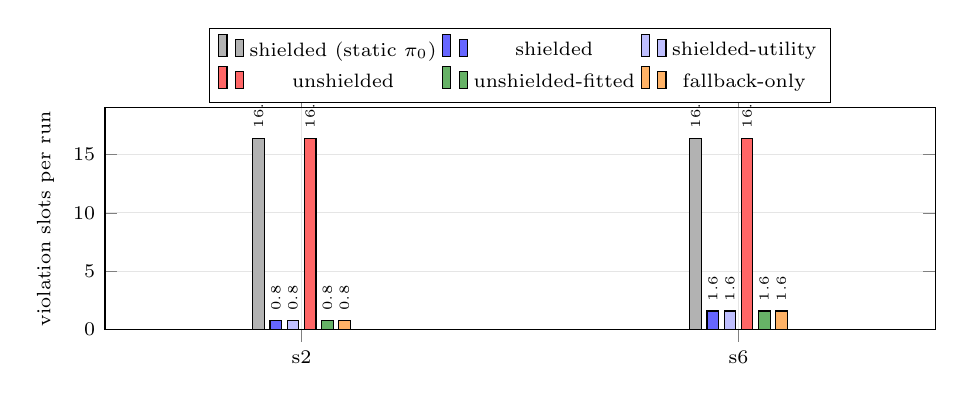
\begin{tikzpicture}
\begin{axis}[ybar, bar width=4.2pt, width=\columnwidth, height=4.4cm,
  ymin=0, ymax=19, ylabel={violation slots per run}, symbolic x coords={s2,s6},
  xtick=data, enlarge x limits=0.45, tick label style={font=\scriptsize},
  label style={font=\scriptsize}, legend style={font=\scriptsize, at={(0.5,1.02)}, anchor=south, legend columns=3},
  nodes near coords, every node near coord/.append style={font=\tiny, rotate=90, anchor=west},
  grid=major, grid style={gray!20}]
\addplot[fill=gray!60] coordinates {(s2,16.4) (s6,16.4)};
\addplot[fill=blue!60] coordinates {(s2,0.8) (s6,1.6)};
\addplot[fill=blue!25] coordinates {(s2,0.8) (s6,1.6)};
\addplot[fill=red!60] coordinates {(s2,16.4) (s6,16.4)};
\addplot[fill=green!50!black!60] coordinates {(s2,0.8) (s6,1.6)};
\addplot[fill=orange!60] coordinates {(s2,0.8) (s6,1.6)};
\legend{{shielded (static $\pi_0$)}, shielded, shielded-utility, unshielded, unshielded-fitted, fallback-only}
\end{axis}
\end{tikzpicture}
\caption{Violation slots in the two surge scenarios (simulation, seeds 1--5). The
first bar uses the static fallback; all others use the capacity-aware fallback.
In s1, s3 and s4 every controller had zero violation slots, and in s5 every
controller had 60.}
\label{fig:fallback}
\end{figure}

\subsection{Utility-based selection}

The two shielded controllers differ only in the selection rule. In every scenario
they had the same violations, fallbacks and delivered throughput (Table~\ref{tab:sim}),
but utility selection reserved 20--32\,\% less bandwidth: 155 against 105\,Mbit/s in
s1, 124 against 91 in s2, 145 against 116 in s4. Among the certified candidates it
chose demand-matched budgets where first-certified took the greedy one whenever
the greedy candidate was certifiable. In the simulator a budget above the offered
load does not change the outcome, so the only measured effect is the smaller
reservation. Since the utility weights are illustrative, this shows that the rule
works as specified, not that these weights are good.

\subsection{H2: model dependence and calibration}

\begin{table}[t]
\caption{Calibration of the latency safety factor $k$. Coverage: fraction of slot--slice points with $k\hat{L}\ge L_{\text{recorded}}$.}
\label{tab:calib}
\centering
\footnotesize
\setlength{\tabcolsep}{3pt}
\begin{tabular}{@{}llcc@{}}
\toprule
Data & Evaluated on & fitted $k$ & $k=1.5$\\
\midrule
\multicolumn{4}{@{}l}{\emph{Simulator}: fitted on seeds 1--5 of s1--s4, s6; $k=1.109$}\\
& held-out seeds 6--10, s1--s4, s6 & 98.3\,\% & 100\,\% \\
& s5 (model mismatch) & 39.6\,\% & 64.7\,\% \\
\midrule
\multicolumn{4}{@{}l}{\emph{Emulated network}: fitted on seeds 1--3 of s1--s3; $k=2.272$}\\
& held-out seeds 4--5, s1--s3 & 98.5\,\% & 95.3\,\% \\
\bottomrule
\end{tabular}
\end{table}

The configured factor $k=1.5$ was chosen, not fitted. On the simulator, the ratio of
recorded to predicted latency (with $k=1$) has a median of 1.00 and a 99th percentile
of 1.11 for every slice in the nominal scenarios, so $1.5$ is about 35\,\% more
pessimistic than necessary there. That pessimism is what causes the 20 uncertified
fallbacks in s3: the model predicts URLLC latency above 1\,ms on the loaded path A
while the simulated latency stays below it, so neither the candidates nor the
fallback can be certified. Re-running the held-out seeds with the fitted $k = 1.109$
removed all 20 fallbacks in s3, with no new violation and no other change in any
scenario.

The fit does not help in s5 (Table~\ref{tab:calib}). There the model assumes 64-byte
URLLC packets while the network sends 1500-byte packets, so the model's error is
structural, not a scale error, and no single factor fits it: coverage drops to
40\,\% with the fitted factor and is only 65\,\% with $k=1.5$. In s5 the shield
certified actions that violated the URLLC intent in all 60 slots, for every
controller.

On the emulated network, the factor fitted on seeds 1--3 was 2.27 and covered
98.5\,\% of the held-out slots, below the 99\,\% rule we had fixed in advance, so
$k=1.5$ was kept. We also did not adopt the simulator's $1.109$, since it would tune
the shield to its own evaluator. The emulated fit is driven by a heavy URLLC tail
(99th percentile of the ratio 3.7, maximum 17), which is related to the open
latency issue below.

\subsection{Emulated network}
\label{sec:meter}

\emph{Meter behaviour.} An earlier emulated campaign showed every controller
exceeding the 0.9 reservation limit in about 20 slots of s2, and metered eMBB slots
delivering 1.07 times their budget on average. A dedicated test isolated the cause
(Table~\ref{tab:meter}): an Open vSwitch meter that is left alone passes exactly its
budget, at any rate (1--70\,Mbit/s), frame size and burst size, but every
modification of the meter passes extra traffic in proportion to its burst size. The
controller modifies the eMBB meter almost every slot, because the certified budget
tracks the measured background. We reduced the meter burst from 0.1\,s to 0.01\,s
and kept the remaining 1\,\% in the model as $\epsilon$ in (\ref{eq:cap}), rather
than programming meters below their budget, which would have hidden the effect from
the shield.

\begin{table}[t]
\caption{Delivered/budget ratio of an Open vSwitch meter, offered 1.5$\times$ its budget, mean over six 1\,s slots (budgets 20 and 50\,Mbit/s gave the same values within 0.002).}
\label{tab:meter}
\centering
\footnotesize
\begin{tabular}{@{}lcc@{}}
\toprule
Meter burst & left unchanged & modified every slot\\
\midrule
0.01\,s & 0.998--0.999 & 1.005--1.006\\
0.1\,s (previous setting) & 1.000 & 1.066\\
1\,s & 1.000 & 1.495--1.497\\
\bottomrule
\end{tabular}
\end{table}

\emph{Scenario s2 after the correction.} Table~\ref{tab:mininet} reports s2 on the
emulated network with the final implementation. The pattern matches simulation:
the unshielded controller had the most violation slots and applied 20 actions per
run that the shield would have rejected, while the shielded controllers, the
capacity-fitted heuristic and the fallback stayed close to zero. Reservation-limit
slots fell from about 20 to about 4 per run after the meter correction; most of the
remainder fall in the first three slots of the surge, and the others exceed the
limit by small amounts consistent with measurement noise. With so few violations,
five seeds are not enough to rank the controllers other than the unshielded one.

\begin{table}[t]
\caption{Emulated network (Mininet/Open vSwitch), scenario s2, seeds 1--5, after the meter correction. Measured values, not ground truth; overload is not observable.}
\label{tab:mininet}
\centering
\footnotesize
\setlength{\tabcolsep}{2.5pt}
\begin{tabular}{@{}lccccc@{}}
\toprule
& shielded & sh.-utility & unshielded & uns.-fitted & fb-only\\
\midrule
Violation slots & $0.6\pm0.9$ & $0.8\pm1.3$ & $4.2\pm1.5$ & $1.2\pm1.8$ & $1.2\pm0.4$\\
Res.-limit slots & 4.0 & 4.6 & 20 & 3.8 & 3.4\\
Shadow rejections & 0 & 0 & 20 & 0 & 0\\
Rejection rate & 0.63 & 0.63 & -- & -- & --\\
Verify, p95 (ms) & 30 & 32 & 4 & 5 & 5\\
eMBB (Mbit/s) & 73.5 & 73.5 & 79.7 & 73.5 & 73.4\\
\bottomrule
\end{tabular}
\end{table}

\emph{Open issue: latency spikes.} In the s1--s3 campaign, which ran before the
meter correction, the URLLC p99 latency exceeded 1\,ms in 43 slots of s1 and 124
slots of s3 (summed over all 25 runs of each scenario), reaching 18.8\,ms on path A, whose propagation delay is 0.2\,ms. The
spikes affected every controller and clustered in individual runs (one shielded s1
run alone had 18 slots in which a slice exceeded its bound), so they are not attributable to the controllers.
On an idle path with the same 100 probes per slot, the per-slot p99 never exceeded
1\,ms (median 0.49\,ms), with or without the counter reads the backend performs each
slot. The spikes therefore require the campaign's traffic or host load, and their
cause is not yet known. For this reason we do not report controller comparisons for
s1 and s3 on the emulated network. Those scenarios have also not yet been repeated
with the meter correction.

\begin{figure*}[t]
\centering
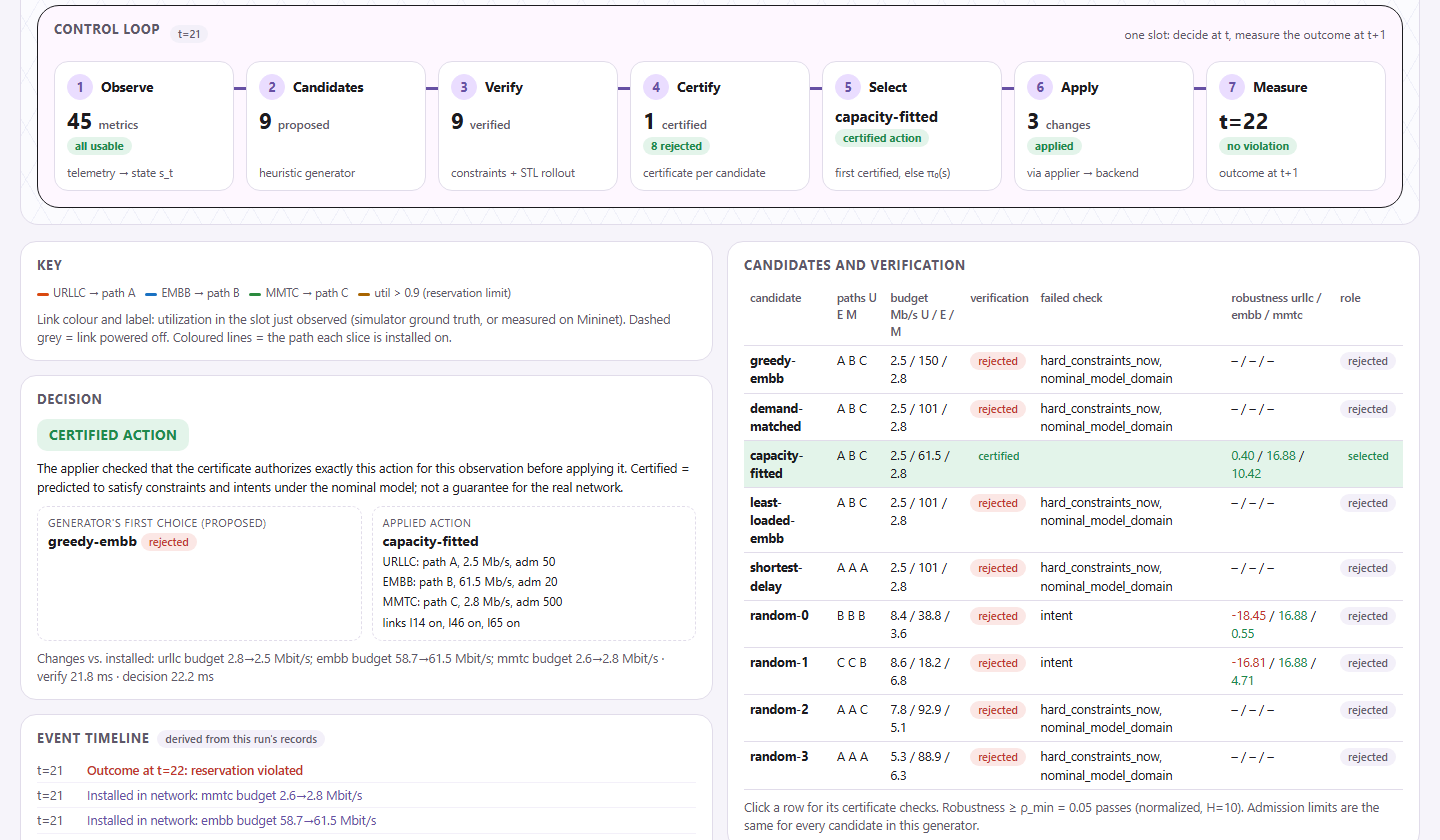
\includegraphics[width=0.92\textwidth]{figures/dashboard_slot.png}
\caption{The prototype's dashboard during one decision (scenario s2, slot 21,
simulation). Top: the seven stages of the slot. Left: the decision card, showing that
the generator's first choice (greedy-embb) was rejected and the certified
capacity-fitted candidate applied. Right: all nine candidates with the failed check
and the robustness per intent; two random candidates were rejected for the URLLC
intent with robustness $-18.5$ and $-16.8$, and the applied one had margins 0.40,
16.88 and 10.42 (all above $\rhomin = 0.05$). Verification of the nine candidates
took 21.8\,ms.}
\label{fig:dashboard}
\end{figure*}

% =====================================================================
\section{Performance Analysis}
\label{sec:analysis}

Table~\ref{tab:hyp} summarizes how the evidence bears on each hypothesis; the rest of
this section analyzes cost, filtering and the sources of the observed behaviour.

\begin{table}[t]
\caption{Hypotheses and evidence}
\label{tab:hyp}
\centering
\footnotesize
\setlength{\tabcolsep}{3pt}
\begin{tabular}{@{}p{0.9cm}p{4.5cm}p{2.3cm}@{}}
\toprule
& Evidence & Verdict \\
\midrule
H1 & s2: 16.4 $\to$ 0.8 violation slots (sim), 4.2 $\to$ 0.6 (emulated); s6: 16.4 $\to$ 1.6; held-out seeds agree & Supported; no gain over the capacity-aware heuristic \\
H2 & s5: certified actions violated URLLC in 60/60 slots; fitted $k$ covers 40\,\% of s5 & Supported \\
H3 & only $\pi_0$ changed: static gives 16.4 (s2, s6) with 20 uncertified fallbacks; capacity-aware gives 0.8 (s2), 1.6 (s6) & Supported \\
\bottomrule
\end{tabular}
\end{table}

\emph{Cost.} Verifying nine candidates, each with a ten-step rollout and three
intents, took 22--33\,ms at the 95th percentile per slot in simulation and about
30\,ms on the emulated network, against 3--5\,ms for the controllers without
verification. Utility selection adds one more rollout per certified candidate
(28--34\,ms). Both are small relative to a one-second slot, but the cost grows
linearly with the number of candidates and the horizon, so a generator that
proposes hundreds of candidates, or a stochastic model that needs many rollouts per
candidate, would change this picture.

\emph{Filtering.} The shield rejected 50\,\% of candidates in s1, 63\,\% in s2 and
s6, 61\,\% in s4 and 67\,\% in s3. In the surge slot shown in Fig.~\ref{fig:dashboard}, eight of nine candidates were
rejected: six for the capacity constraint together with the model's validity range,
and two random candidates for the URLLC intent. Measured against the formulation's Constraint 2, these are high rejection
rates, but they are rates for deliberately poor and random proposals, not for a
trained generator.

\emph{Where the safety came from.} Three observations together locate the source of
the improvement. With the static fallback the shield did not help; with the
capacity-aware fallback it did; and a capacity-aware heuristic achieved the same
result without the shield. The safety in the surge scenarios therefore comes from
having a decision that accounts for measured background load. What the shield adds
is that this property holds for whatever candidates are proposed, which the shadow
counts make concrete: 20 rejected actions per s2 run for the greedy generator, and
none for the heuristic.

\emph{Reaction lag.} Every controller pays for the first slot of a surge, because
the decision for that slot is made before the surge is measured. The shield
evaluates candidates against the current measurement and a constant forecast; it
cannot anticipate an event that the measurements do not show. Actuation delay (s6)
adds about one further slot, because the effect of a certified action falls outside
the window that was checked.

\emph{Conservatism versus safety.} In s3 and s4 the shield refused to certify
anything for 20 and 13 slots, although nothing would have been violated. In s3 this
is the pessimism of $k=1.5$ and disappears with a calibrated factor. In s4 it is the
intended behaviour on frozen or missing telemetry, at a cost of about 3\,\% eMBB
throughput relative to the unshielded controller. In s5 the opposite happened: the
model was optimistic, and the shield certified actions that were not safe. Both
failure directions are properties of the model, not of the verification logic.
